\begin{figure}[t]
    \centering
    \begin{adjustbox}{max size={.6\textwidth}{.6\textheight}}
    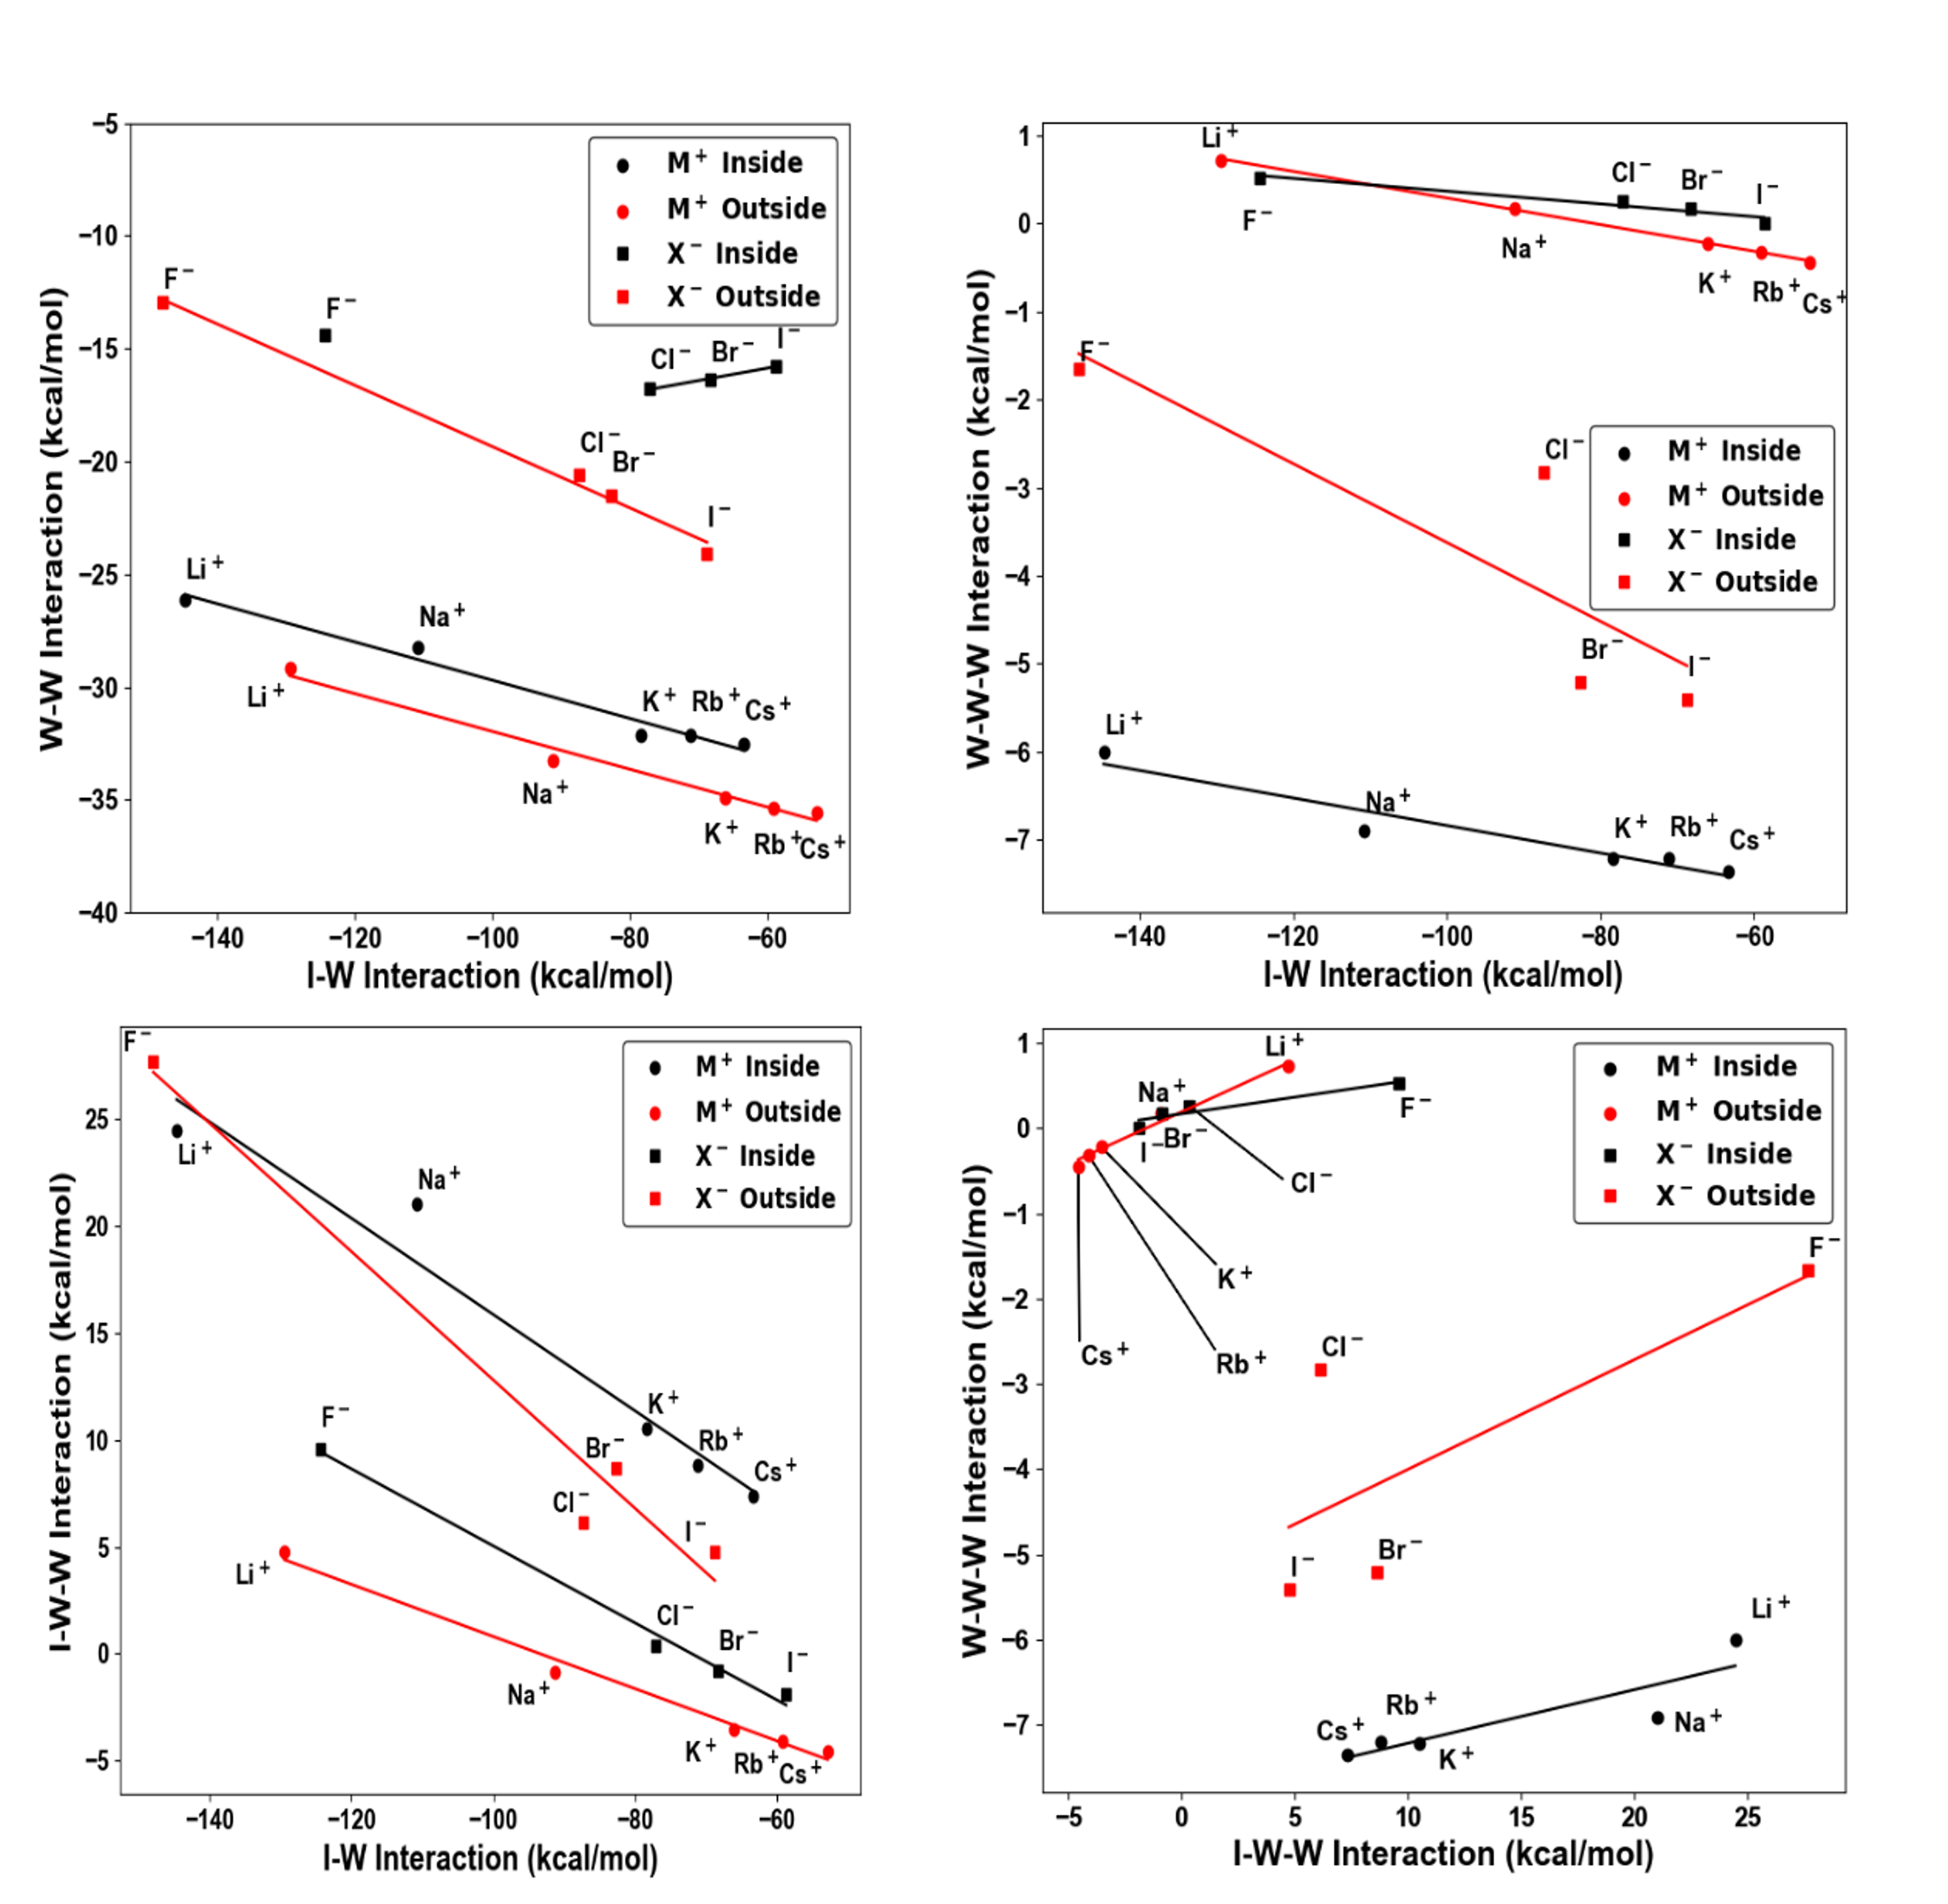
\includegraphics[width=\textwidth]{Figures/Chapter_3/figure_9_combined.png}
    \end{adjustbox}
    \begin{spacing}{1.0}
  \caption[Correlations between the various interactions for the \ce{Z^{+/-}(H2O)9}, \ce{Z} = \ce{M^+} (\ce{Li^+}, \ce{K^+}, \ce{Cs^+}) and \ce{Z} = \ce{X^-} (\ce{Cl^-}, \ce{Br^-}, \ce{I^-}) clusters. (a) Top left panel: (W-W) vs. (I-W), (b) top right panel: (W-W-W) vs. (I-W), (c) bottom left panel: (I-W-W) vs. (I-W) and (d) bottom right panel: (I-W-W) vs. (W-W-W) interactions.]{Correlations between the various interactions for the \ce{Z^{+/-}(H2O)9}, \ce{Z} = \ce{M^+} (\ce{Li^+}, \ce{K^+}, \ce{Cs^+}) and \ce{Z} = \ce{X^-} (\ce{Cl^-}, \ce{Br^-}, \ce{I^-}) clusters. (a) Top left panel: (W-W) vs. (I-W), (b) top right panel: (W-W-W) vs. (I-W), (c) bottom left panel: (I-W-W) vs. (I-W) and (d) bottom right panel: (I-W-W) vs. (W-W-W) interactions.}\label{fig:MBE_II_9}
  \end{spacing}
\end{figure}